\section{Satellite Based Augmentation Systems}
	The average positional error we get by using pseudoranges observed from four or more satellites is about 10 m. By studying the error budget in Table 9.6, we recognize that the largest error contribution comes from the ionospheric delay.
	
	When the positional error is brought down to 1-2 meters, GPS becomes very useful for flight navigation (category I landing), transportation, and farming.
	
	There is always a risk that the computed position is incorrect as a result of anomalous GPS behavior or environmental degradation. The user has no ideas of the actual error and how the situation will alter in the near future. Consequently many applications that require a high level of confidence in the computed position can not use GPS alone. Satellite based augmentation systems (SBAS) assure a given position accuracy and level of confidence.
		
	Such ideas are now realized by WAAS in the US and by EGNOS in Europe: The Wide Area Augmentation System (operational since 2003), the European Geostationary Navigation Overlay System (operational since October 2009). WAAS is supported by Federal Aviation Administration and EGNOS is supported by Eurocontrol, both avionics institutions.
	\begin{figure}
		\centering
		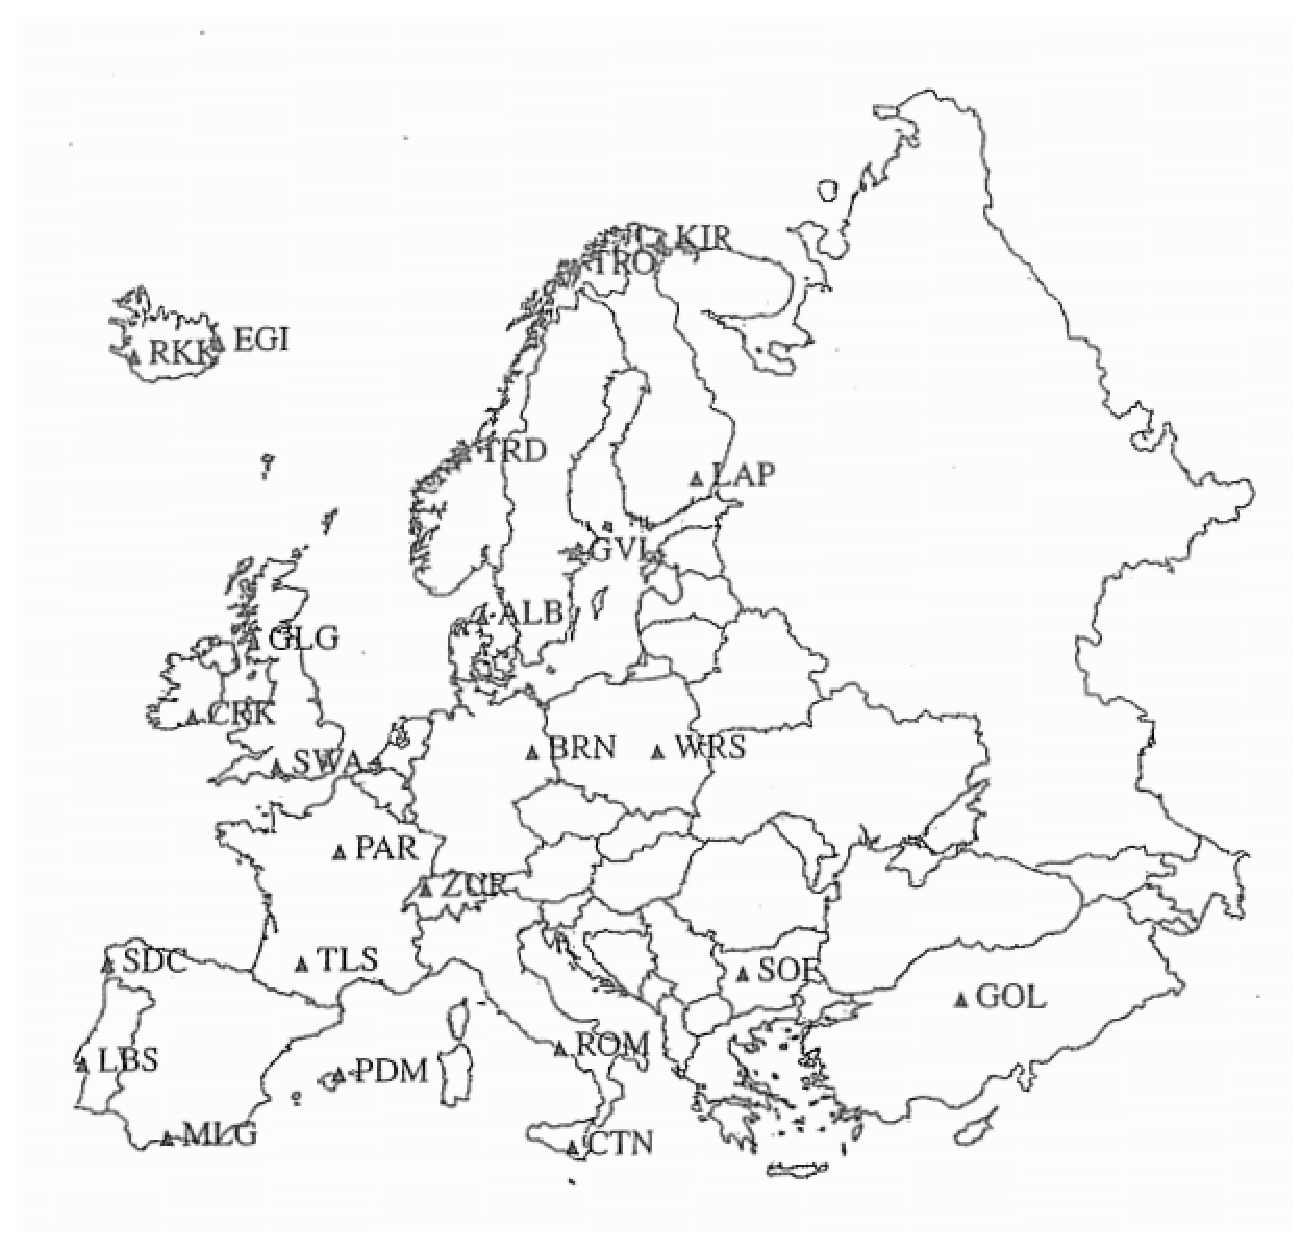
\includegraphics[width=0.7\linewidth]{TeX_files/Part03/chapter09/image/9-20}
		\caption{Positions of European EGNOS RIMS}
		\label{fig:9-20}
	\end{figure}

	The MSAS in Japan, the GAGAN system in India, and the SNAS system in China are currently regional systems. The need is commonly recognized to establish cooperation and coordination among different systems so that their implementation becomes and part of a seamless world-wide navigation system.
	
	We want to emphasize that these Satellite Based Augmentation Systems (SBAS) are conceptually different from Differential GPS. In DGPS a master station computes corrections to the observed pseudoranges which are transferred to one or more rover stations via a land mobile radio-network. Typical transmission ranges are shorter than 50-200km; they are limited by the curvature of the Earth and the transmitting effect. The corrections become more and more unreliable, the longer the baseline is between master and rover.In SBAS the final positional accuracy is intentionally aimed at being uniform over a wide area of land. Today SBAS consistently delivers positional accuracies better than 1 m. This number competes with many differential services.
	
	\subsection{Ranging and Integrity Monitoring Station}
		In the following we will interchangeably use WAAS and EGNOS to illustrate various aspects of SBAS.
		
		In an SBAS, single frequency receivers at known positions track all visible GPS (and GLONASS) satellites and next estimate the ionospheric delay / based on dual frequency observations. When fully deployed EGNOS will have 34 such Ranging and Integrity Monitoring Stations (RIMS). Their geographical distribution is depicted in Figure \ref{fig:9-20} and the station coordinates are listed in Table \ref{tab:9.7}.
		\begin{table}
			\centering
			\caption{List of RIMS positions. Latitude $\varphi$ is positive on the northern and negative on the southern hemisphere. Longitude $\lambda$ is positive to the east of Greenwich and negative to the west.}
			\label{tab:9.7}
			\begin{tabular}{llll}			
				\hline Code & Name & $\varphi$ & $\lambda$ \\ 
				\hline ACR	& Azores Islands & 38.51 & -28.62 \\
					   ALB  & Aalborg & 57.10 & 9.90 \\
					   BRN	& Berlin & 52.32 & 13.25 \\
					   CIN 	& Catania & 37.47 & 15.07 \\
					   CNR 	& Canarias & 27.95 & -15.38 \\
					   CRK 	& Cork & 51.85 & -8.50 \\
					   DAB 	& El Daba & 31.02 & 28.47 \\
					   DJA 	& Djerba & 33.87 & 10.77 \\
					   EGI 	& Egilsstadir & 65.28 & -14.40 \\
					   GLG  & Glasgow & 55.70 & -4.10 \\
					   GOL  & Golbasi & 39.63 & 32.80 \\
					   GVL  & Gavle & 60.67 & 17.13 \\
					   HBK  & Hartebeeshoek & -25.88 & 27.70 \\
					   KIR  & Kirkenes & 69.68 & 29.92 \\
					   KOU  & Kourou & 5.17 & -52.68 \\
					   LAP  & Lappeenranta & 61.53 & 27.55 \\
					   LSB  & Lisbon & 38.78 & -9.13 \\
					   MAD  & Madere & 32.75 & -16.70 \\
					   MLG  & Malaga & 36.68 & -4.52 \\
					   MON  & Moncton & 46.07 & -64.78 \\
					   NOU  & Nouackhott & 18.09 & -15.58 \\
					   PAR  & Paris & 48.83 & 2.33 \\
					   PDM  & Palma de Mallorca & 39.57 & 2.73 \\
					   RKK  & Reykjavik & 64.13 & -21.93 \\
					   ROM  & Roma & 41.80 & 12.58 \\
					   SDC  & Santiago de Compostela & 42.92 & -8.42 \\
					   SOF  & Sofia & 42.80 & 23.42 \\
					   SWA  & Swanwick & 50.88 & -1.28 \\
					   TLS  & Toulouse & 43.42 & 1.50 \\
					   TRD  & Trondheim & 63.45 & 10.90 \\
					   TRO  & Troms0 & 69.67 & 18.95 \\
					   WRS  & Warszawa & 52.22 & 21.07 \\
					   ZUR  & Zurich & 47.45 & 8.57 \\
				\hline 
			\end{tabular} 
		\end{table}
		However, the signals will do more than fix a position. They will provide information about the accuracy of position measurements delivered by GPS. This information, or integrity data, will be modulated onto the ranging signal. It will include accurate information on the position of each GPS and GLONASS satellite, the accuracy of the atomic clocks on board the satellites, and disturbances within the ionosphere. The special EGNOS receiver will decode the signal to give a more accurate position and error estimate than is possible with GPS or GLONASS alone.
		
		Observations are taken every second and transmitted to four Mission Control Centers (MCC) that determine the integrity, pseudorange differential correction for each monitored satellite, ionospheric delays and generate ephemerides for the GEOs. A network will connect them to the ground stations that up-link the information to the GEO satellites.
		
		The EGNOS signal will be broadcast by GEO satellites. Unlike the GLONASS and GPS satellites, these will not have signal generators on board. A transponder will transmit signals up-linked to the satellites from the ground, where all the signal processing will take place. The current GEOs and their PRN numbers are collected in Table 9.8. All satellites are operated by Inmarsat, except Artemis which is operated by ESA.
		
		In pole-close areas these GEO satellites are seen at low elevation angles (20° at Aalborg, see Figure 9.30). Therefore low buildings and other objects are likely to shadow for the GEO satellites and no correction signal is received. To repair this situation ESA provides access to the EGNOS signals via the internet. The service is called SISNeT.
		\begin{table}[h]
			\centering
			\caption{WAAS and EGNOS GEO satellites and their PRN numbers}
			\label{tab:9.8}
			\begin{tabular}{cccc}
				\hline
				SBAS & Satellite & PRN & Longitude \\ 
				\hline
				WAAS & AOR-W & 122 & $54^\circ$ W \\ 
					 & POR & 134 & $178^\circ$ E \\ 
				EGNOS & AOR-E & 120 & $15.^\circ$ W \\ 
					 & Artemis & 124 & $21.5^\circ$ E \\ 
					 & IOR-W & 126 & $25^\circ$ E \\
				\hline 
			\end{tabular} 
		\end{table}
		  
		A Monitoring Station (RIMS) computes the positions of each GPS and GLONASS satellite. It compares accurate positions with measurements obtained from the satellites’ signals. The RIMS then sends the data to the master control centers. The master control centers determine position inaccuracies due to disturbancesin the ionosphere. All the deviation data are then incorporated into a signal and sent securely to the up-link stations, which are widely spread across Europe. The up-link stations send the signal to the three EGNOS GEO satellites which then transmit it to GPS and GLONASS users with an SBAS receiver.
		
		Considerable redundancy is built into EGNOS so that the service can be guaranteed at practically all times. At any one time, one control center will be “ the master,” with another on stand-by. Only three up-link stations are needed to operate EGNOS, one for each satellite. The other three are in reserve.
		
		EGNOS offers
		\begin{itemize}
			\item a correction of the pseudorange PRC($t_{of}$)
			\item an ionospheric delay correction $I_{slant}$, and
			\item an integrity measure $\sigma^2_{UDRE}$.
		\end{itemize}
		A user of SBAS obtains the ionospheric delay corrections as a vertical delay estimate at specified ionospheric grid points (IGP). They are defined for a grid with 5° resolution in latitude and longitude near the.Equator and coarser resolution near the poles.
		
		The vertical ionospheric delay is estimated at these grid points. This is a truth with a small modification. The value is not valid at the grid point itself but at a point 350 km above; this leads to a complication for the user. The reason is to define the ionospheric delay as a single layer delay at this height above the WGS 84 ellipsoid.
		
		The ionospheric delay at a grid point is estimated .from the neighboring RIMS by a geometric and statistic interpolation, see Walter et al. (2000). The preliminary receiver position is given as (X , Y, Z), converted if necessary from $(\varphi,\lambda,h)$. Knowing also the satellite position $(X^s , Y^s , Z^s )$ we determine $(\varphi,\lambda)$ for the ionospheric pierce point (IPP). This IPP is the intersection of the line segment between the receiver and satellite with the parallel surface to the WGS 84 ellipsoid at the altitude of H = 350 km. This computation is done by the M-file ipp. The $(\varphi,\lambda)$ for the IPP is used to compute the ionospheric delay in message type 26. 
	
	\subsection{SBAS Messages and Their Generation}
		For both WASS and EGNOS, the key document that describes the signal specification for SBAS is RTCA/DO-229C (2001), Appendix A. Inter-operability makes it likely that all future SBAS will use the same model. Table 9.9 surveys the message types, including signal characteristics, contents and format for SBAS integrity and correction data. Typical message types tracked are: 2-5, 18, 24, and 26. In the sequel we only mention these types.
		
		The baseline data rate will be 250 bits per second (bps). The data will always be rate 1/2 com olutional encoded with a forward error correction (FEC) code. Therefore, the GPS receiver processes 500 symbols per second (sps). The convolutional coding will be constraint length 7 as standard for Viterbi decoding.
		
		The SBAS data are modulated on the LI signal which is transmitted from a GEO satellite as a GPS-type modulation. The rate is 500 sps which is 10 times faster than the navigation message. The SBAS data are added modulo-2 to a 1023-bin PRN code and then bi-phase shift-keyed modulated onto the carrier at a rate of 1.023 Mchips per second. The 500 sps will be synchronized with the 1 kHz C/A code epochs.
		
		The SBAS codes are identified in three ways: PRN number, G2 delay in chips, and the initial G2 state. The PRN number starts with 120 instead of 1. The actual code is defined by the initial G2 register setting. For use of the G 2 sequence, see page 17. For details in general, see RTCA/DO-229C (2001).
		
		The 24 bit cyclic redundancy check (CRC) parity is generated for the polynomial
		\begin{equation*}
			g(X)=(1+X)p(X)
		\end{equation*}
		where
		\begin{equation*}
			p(X)=X^{23}+X^{17}+X^{12}+X^{11}+X^9+X^8+X^7+X^5+X^3+1
		\end{equation*}
		
		The data flow is made up of blocks of 250 bps. Each block starts with an 8 bit preamble, next a 6 bit message type identifier, and a 212 bit data field, and finally 24 bits for CRC parity check. The transmission time for a block is 1s.
		\begin{table}[h]
			\centering
			\caption{SBAS Message Types}
			\label{tab:9.9}
			\begin{tabular}{rl}
				\hline
				0 & Don’t use for safety applications \\
				1 & PRN Mask assignments, set up to 51 of 210 bits\\
				2-5 & Fast corrections\\
				6 & Integrity information\\
				7 & Fast correction degradation factor\\
				8 & Reserved for future messages\\
				9 & GEO navigation message (X,Y,Z,time,etc.)\\
				10 & Degradation Parameters\\
				11 & Reserved for future messages\\
				12 & WAAS Network Time/UTC offset parameters\\
				13-16 & Reserved for future messages\\
				17 & GEO satellite almanacs\\
				18 & Ionospheric grid point masks\\
				19-23 & Reserved for future messages\\
				24 & Mixed fast corrections/long term satellite error corrections\\
				25 & Long term satellite error corrections\\
				26 & Ionospheric delay corrections\\
				27 & WAAS Service Message\\
				28 & Clock-Ephemeris Covariance Matrix Message\\
				29-61 & Reserved for future messages\\
				62 & Internal Test Message\\
				63 & Null Message\\
				\hline
			\end{tabular} 
		\end{table}
		Next we briefly describe selected SBAS message types. Details are left out as we indicate how a user obtains corrections to his observations. Then he computes a receiver position at meter-level:
		
		Message 1 allocates a PRN number to the correction slot in the block format described by a 2 bit Issue Of Data PRN. This IODP is a unique identifier for a PRN number.
		
		Message 2-5 contains the fast data set. The block starts with the 2 bit IODP, an 8 bit preamble, a 6 bit message type identifier (values can be 2, 3, 4, or 5), and a 2 bit issue of data fast (IODF). Next follows the fast data set for 13 satellites: 12 bits for the fast pseudorange correction PRC and 4 bits for user differential range error indicator (UDREI).The block ends with 24 parity bits, in total 250 bits. The fast data set for the next 13 satellites are contained in the following block.
		
		The PRC value is between —256 and +256—$\dfrac{1}{8}$ with a resolution of $\dfrac{1}{8}$m. The rangerate correction RRC of the fast correction is computed as the difference between the current PRC and the previous one divided with the time interval between the two values. The time of applicability $t_{of}$ is identical to the transmission time of the first bit in the block from the GEO.
		\begin{table}[h]
			\centering
			\caption{Interpretation of the 4 bit user differential range error indicator}
			\label{tab:9.10}
			\begin{tabular}{ccc}
				\hline 
				Bit value & UDRE[m] & $\sigma^2_{UDRE}[m^2]$ \\ 
				\hline 
				0 & 0.75 & 0.0520\\
				1 & 1.00 & 0.0924\\
				2 & 1.25 & 0.1444\\
				3 & 1.75 & 0.2830\\
				4 & 2.25 & 0.4678\\
				5 & 3.00 & 0.8315\\
				6 & 3.75 & 1.2992\\
				7 & 4.50 & 1.8709\\
				8 & 5.25 & 2.5465\\
				9 & 6.00 & 3.326\\
				10 & 7.50 & 5.197\\
				11 & 15.00 & 20.79\\
				12 & 50.00 & 231.0\\
				13 & 150.00 & 2078\\
				14 & Not monitored & Not monitored\\
				15 & Do not use & Do not use\\
				\hline
			\end{tabular} 
		\end{table}
		The fast correction to the pseudorange for a given PRN is
		\begin{equation}\label{eq:9.51}
			PR_{corrected}(t)=PR_{observed}(t)+PRC(t_{of})+PRC(t_{of})(t-t_{of})
		\end{equation}
		The RRC computation must time-out if there is no PRC for 8s.
		
		The 4 UDRE indicator bits are interpreted according to Table \ref{tab:9.10}.
		
		Message 6 indicates the integrity; it is already included in messages 2-5. It is used if one satellite has an alert.
		
		Message 18 The total number of ionospheric grid points (IGP) is large. All mesh points have by default a bit set to 0. By changing this bit to 1 for an IPP, the message indicates that ionospheric correction information is available.
		
		Message 26 gives the ionospheric delay correction in form of a vertical delay, relative to an L1 signal, and the accuracy $\sigma^2_{GIVE}$ at the defined IGPs, GIVE is short for grid ionospheric vertical error.
		
		With known user position, we can identify four IGPs spanning the quad in which the user is located. These IGPs can be looked up in the message and for each IGP we read a 9 bit vertical delay I in the range 0-63.75 m with a resolution of 0.125 m.
		
		Now $I_{weighted}$ is computed as a weighted mean of the four values of I at the IGPs.
		\begin{equation}\label{eq:9.52}
			I_{weighted}=\sum^4_{i=1}\omega_iI_i
		\end{equation}
		\begin{table}[h]
			\centering
			\caption{Interpretation of the 4 bit GIVE Indicator}
			\label{tab:9.11}
			\begin{tabular}{ccc}
				\hline 
				Bit value & GIVE[m] & $\sigma^2_{GIVE}[m^2]$ \\
				\hline
				0 & 0.3 & 0.0084\\
				1 & 0.6 & 0.0333\\
				2 & 0.9 & 0.0749\\
				3 & 1.2 & 0.13\\
				4 & 1.5 & 0.21\\
				5 & 1.8 & 0.30\\
				6 & 2.1 & 0.40\\
				7 & 2.4 & 0.53\\
				8 & 2.7 & 0.67\\
				9 & 3.0 & 0.83\\
				10 & 3.6 & 1.19\\
				11 & 4.5 & 1.87\\
				12 & 6.0 & 3.32\\
				13 & 15.0 & 20.78\\
				14 & 45.0 & 187.08\\
				15 &Not monitored & Not monitored \\
				\hline
			\end{tabular} 
		\end{table}
		with weights adding to 1:
		\begin{equation*}
			\omega_1 =xy,\,\omega_2=(1-x)y,\,\omega_3=(1-x)(1-y),\,\omega_4=x(1-y)
		\end{equation*}
		where JC is the relative difference in longitude for the IPP relative to the western IGPs and y is the relative difference in latitude to the southern IGPs.
		
		The final correction $I_{slant}$ to the observed pseudorange includes an obliquity factor:
		\begin{equation}\label{eq:9.53}
			I_{slant} = -I_{weighted}/\sqrt{1-(\dfrac{R\cos h}{R+H})^2}
		\end{equation}
		where R = 6378.136 km, H = 350 km, and h is the satellite elevation angle in radians.Given the variance $\sigma^2_{GIVE}$ in Table \ref{tab:9.11} we can compute error variances in unit of $m_2$:
		User User Ionospheric Vertical 
		\begin{equation}\label{eq:9.54}
			\sigma^2_{UIVE}=\sum^4_{i=1}\omega_i\sigma^2_{GIVE}
		\end{equation}
		and User Ionospheric Range Error
		\begin{equation}\label{eq:9.55}
			\sigma^2_{UIRE}=\dfrac{\sigma^2_{UIVE}}{1-(\dfrac{R\cos h}{R+H})^2}
		\end{equation} 
	
	\subsection{Summary of the SBAS Corrections}
		Via SBAS the user is informed about individual pseudorange corrections for clocks and orbit errors (messages 2-5), ionospheric delays (message 26) and integrity (messages 2-5 and 6). Those indicate the quality of GPS positioning. . Users must compute their own (local) tropospheric delay correction.
	
	\subsection{easy13}\label{subsec:easy13}
		The usual position determination involves four unknowns: receiver coordinates (X,Y,Z)and receiver clock offset. If we can observe five or more pseudoranges, the redundant pseudoranges could check consistency among the observations— the fundamental principle behind Receiver Autonomous Integrity Monitoring (RAIM).
		
		easyl 3 describes a technique for RAIM. Horizontal and vertical protection levels (HPL and VPL) are key concepts. Necessarily, some theory is needed to motivate the procedures. (We will return to this topic with some further graphical illustrations in easyl 4.)
		
		RAIM is a major technique for GNSS in many safety-critical applications. It has been with us since about 1990. Much of the following material relies on the work by Pervan (1996).
		
		Let the 4 by 1 vector of unknowns be denoted x. The m by 1 vector of observations is b. A is an m by 4 matrix and the pertinent linear observation equation is:
		\begin{equation}\label{eq:9.56}
			Ax = b + e\quad and\quad \sum_b = \sigma^2_bI
		\end{equation}
		The vector e contains residual errors, in the observations and $\sum_b$ is the given covariance matrix for the pseudoranges.
		
		RAIM is activated for $m\geq5$. Presently there is no standardized RAIM method; so,we choose to present the simplest RAIM fault detection based on the residual norm $\Arrowvert e \Arrowvert$ .
		
		We define the position error as
		\begin{equation}\label{eq:9.57}
			\delta x = x - \hat{x} = x - (A^TA)^{-1}A^Tb = x-(A^TA)^{-1}A^T(Ax-e) = (A^TA)^{-1}A^Te.
		\end{equation}
		The estimated residuals $\hat{e}$ equal the observations b minus the estimated observations
		\begin{equation}\label{eq:9.58}
			\hat{e} = b-A\hat{x} = (I-A(A^TA)^{-1}A^T)b = Sb.
		\end{equation}
		this residual vector $\hat{e}$ solves $A^T(b-A\hat{x})=0$,the normal equations for $\hat{x}$.The components of $\hat{e}$are dependent as they are computed according to \ref{eq:9.58}.The covariance matrix for $\hat{e}$ is
		\begin{equation}\label{eq:9.59}
			\sum_{\hat{e}} = S \sum_{b}S^T= \sigma^2_bSS^T=\sigma^2_bS
		\end{equation}
		Note that $S=I-A(A^TA)^{-1}A^T$is a projector and thus idempotent:$S=S^2$.The covariance $\sum_b$ is diagonal,while $\sum_{\hat{e}}$ is a full matrix!;
		
		In order to identify the probability distribution of the residuals we introduce a further transformation of the vector $\hat{e}$.
		
		The projector S is symmetric and m by m,but singular.I-S projects onto the column space when S projects onto the left nullspace of A. We will transform the observation equations in such a way that the covariacne maotrix $\sum_{\hat{e}}$ is changed into an identity matrix.
		\begin{figure}
			\centering
			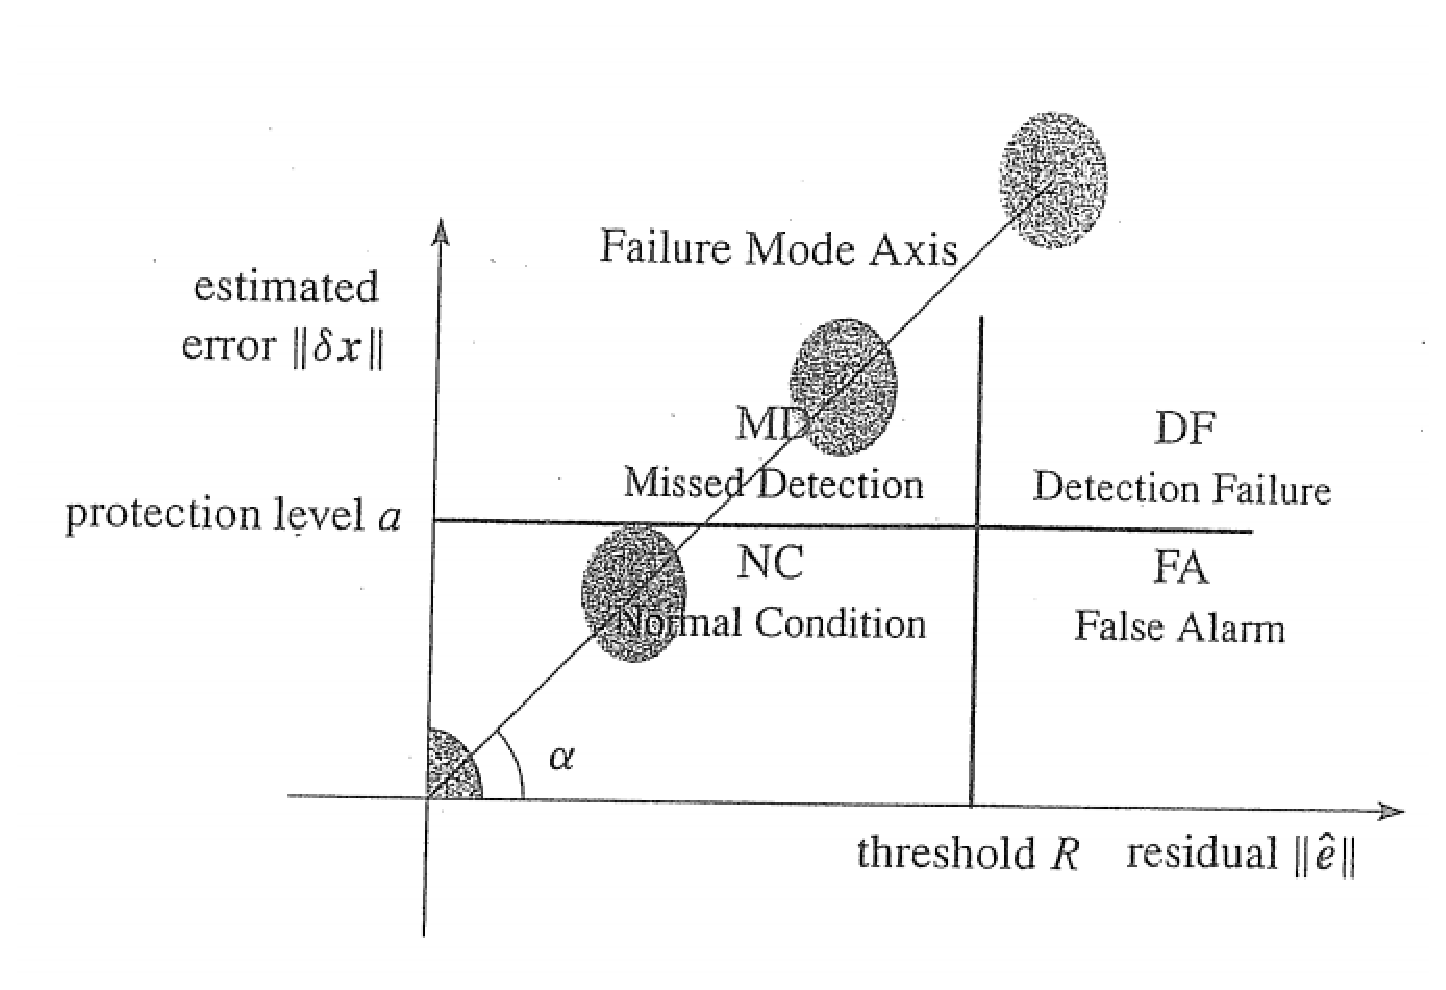
\includegraphics[width=0.7\linewidth]{TeX_files/Part03/chapter09/image/9-21}
			\caption{Four basic RAIM states}
			\label{fig:9-21}
		\end{figure}
		Start with $S = V\Lambda V^T$, where the eigenvalue matrix $\Lambda$ has m — 4 ones and 4 zeros.The orthogonal columns of V are the eigenvectors of S. Let the rows of T contain the m—4 eigenvectors with eigenvalue 1, so that $S=T^TT$and$TT^T=l_{m-4}$.
		
		Transform the residual vector $\hat{e}$ to $e^*=T\hat{e}/\sigma_b$.Then the covariance matrix $\sum^*$for $e^*$is the identity:
		\begin{align}\label{eq:9.60}
		E{e^*(e^*)^T}&=\dfrac{1}{\sigma^2_b}TE{\hat{e}\hat{e}^T}T^T=\dfrac{1}{\sigma^2_b}T\sigma^2_bST^T=TST^T \\
		&=T(T^TT)T^T=(TT^T)(TT^T)=I_{m-4}.
		\end{align}
		The components of $e^*$.are now independent standard gaussians, with zero mean and variance 1. The sum of squares has the $\chi^2$ distribution:
		\begin{equation}\label{eq:9.61}
			\Arrowvert e^* \Arrowvert^2\sim \chi^2_{m-4},\quad m>4
		\end{equation}
		
		Figure \ref{fig:9-21}illustrates four basic RAIM states. In Figure \ref{fig:9-21} they become four possible outcomes or “cases” experienced when using RAIM: normal error condition (NC), missed detection (MD), detection failure (DF), and false alarm (FA).
		
		A residual threshold R can be set analytically using \ref{eq:9.61} to achieve any desired probability of false alarm, $\Arrowvert e^*\Arrowvert > R$;(FA) under normal error conditions (NC):
		\begin{equation}\label{eq:9.62}
			P(FA|NC)=\dfrac{1}{2^{(m-4)/2}\Gamma(\dfrac{m-4}{2})}\int^\infty_{R^2/\sigma^2_b}s^{(m-6)/2}e^{-s/2}ds.
		\end{equation}
		Given the values of $m — 4$ and $F(FA|NC)$ we may solve (9.62) for R. The situation is depicted in Figure \ref{fig:9-22}. The M-code for plotting this figure is contained in the file fap.m.
		
		In Figure \ref{fig:9-21} a horizontal line constraint is drawn to represent the protection level a.Note that for small failure magnitudes, this accuracy specification might not be breached.
		\begin{figure}
			\centering
			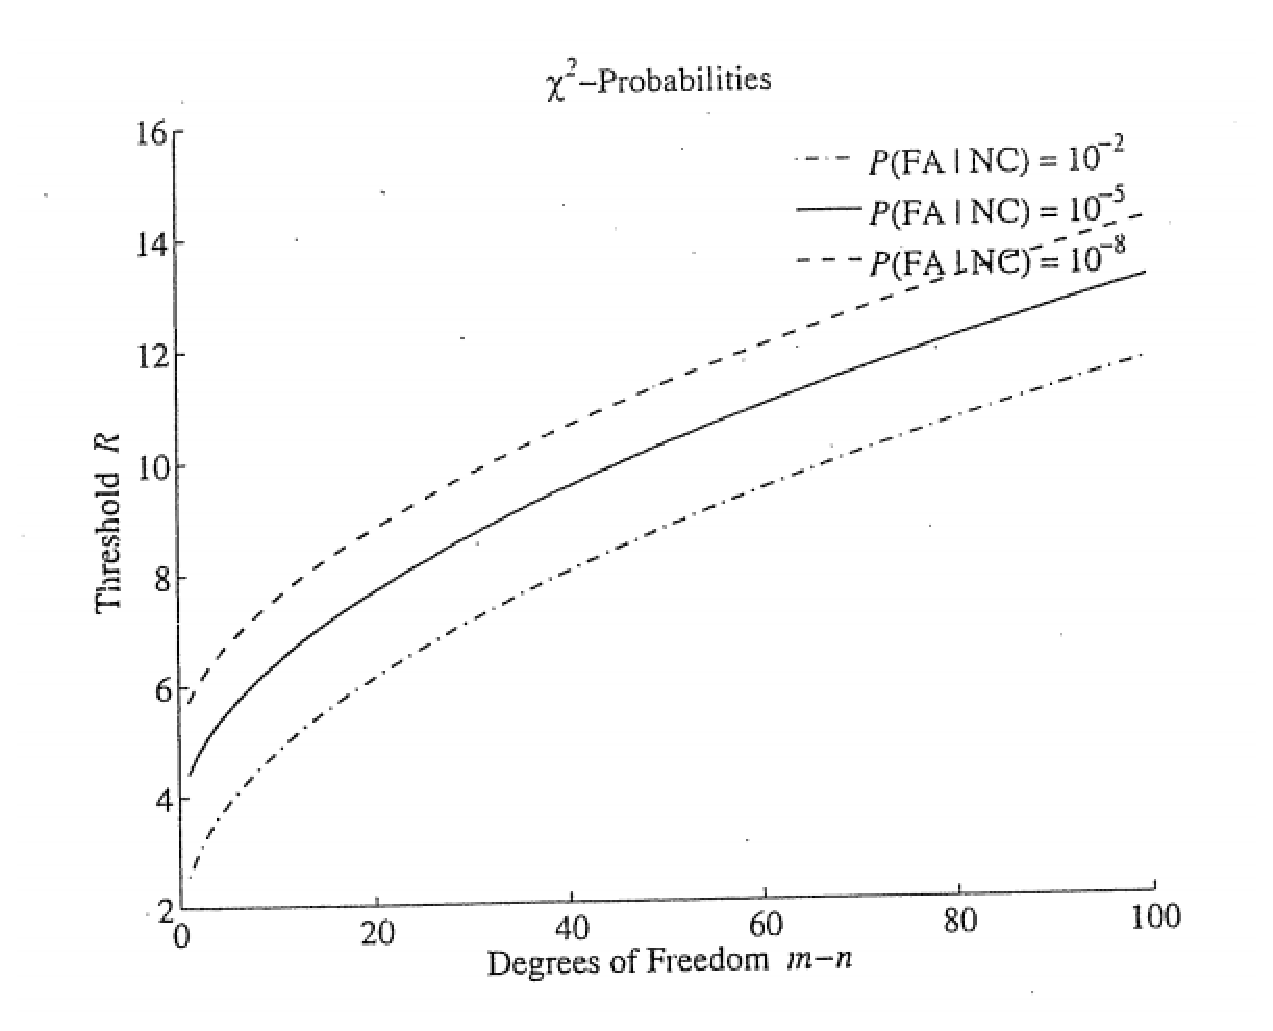
\includegraphics[width=0.7\linewidth]{TeX_files/Part03/chapter09/image/9-22}
			\caption{Probability of false alarm}
			\label{fig:9-22}
		\end{figure}
		In case that the position error $\delta x$ exceeds a predefined protection level a, but $\Arrowvert \hat{e} \Arrowvert <R$——the residual threshold R determined from \ref{eq:9.62}— a missed detection (MD) has occurred.This is case II in Figures \ref{fig:9-21} and \ref{fig:9-24}. The corresponding probability is defined as
		\begin{equation}\label{eq:9.63}
			P(MD)=P(\Arrowvert \hat{e} \Arrowvert < R,\Arrowvert \delta x \Arrowvert >a).
		\end{equation}
		In general there is correlation between $\Arrowvert \hat{e} \Arrowvert$ and $\Arrowvert \delta x \Arrowvert$. We must quantify the degree of this correlation in order to  demonstrate the integrity monitoring capability of RAIM-based fault detection. The result is given later in equation \ref{eq:9.68}.
		
		In \ref{eq:9.57} the position error is $\delta x = (A^TA)^{-1}A^Te$. $\delta x$ is defined in the (X,Y,Z)system. In practice a local topocentric system $\delta x_{ENU} = (e,n,u)$ is more appropriate.This only requires multiplication by the orthogonal transformation matrix $F^T$:
		\begin{equation}\label{eq:9.64}
			F^T = 
			\begin{bmatrix}
			-\sin \lambda & \cos \lambda & 0 \\
			-\sin \varphi \cos \lambda & -\sin \varphi \sin \lambda & \cos \varphi \\
			\cos \varphi \cos \lambda & \cos \varphi \sin \lambda & \sin
			\end{bmatrix}
		\end{equation}
		In the following discussion we only consider the three coordinates (X,Y,Z). So we delete the last column of A and get a new matrix $A_0=A(:,1:3)$.Similarly we delete the last element of $\delta x$ and define $\delta x_0 = \delta x(1:3)$. Hence
		\begin{equation}\label{eq:9.65}
			\delta x_{ENU} = 
			\begin{bmatrix}
			e \\ n \\ u
			\end{bmatrix}
			= F^T\delta x_0 = F^T(A^T_0A_0)^{-1}A^T_0e = Me
		\end{equation}
		Note that rows 1 and 2 of the 3 by m matrix M relate to easting and northing. Finally we define $M_0 = M(1:2,:)$.
		\begin{figure}
			\centering
			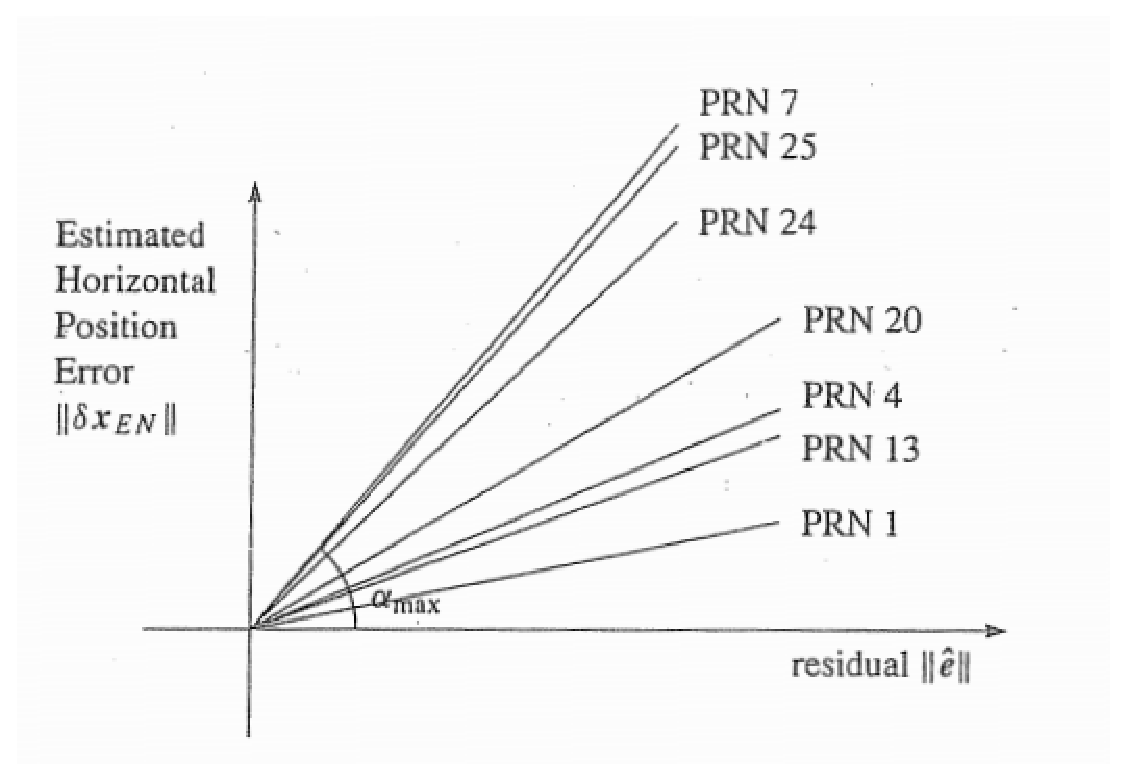
\includegraphics[width=0.7\linewidth]{TeX_files/Part03/chapter09/image/9-23}
			\caption{Characteristic slopes for seven visible satellites. The coordinates of the PRNs are given in Table 9.4.}
			\label{fig:9-23}
		\end{figure}
		
		Imagine now a failure of magnitude $\beta$ in satellite i($\beta$is placed as the $i$ th component):
		\begin{equation}\label{eq:9.66}
			e=
			\begin{bmatrix}
			0 & \ldots & 0 & \beta & 0 & \ldots & 0
			\end{bmatrix}^T
		\end{equation}
		We compute the norm squared for this special choice of e:
		\begin{equation*}
			\Arrowvert \delta x_{EN} \Arrowvert^2 = e^TM^T_0M_0e = (m^2_{1i}+m^2_{2i})\beta^2
		\end{equation*}
		From \ref{eq:9.58} we recall $\hat{e} = Sb$. Then $S^TS=S$leads to
		\begin{equation*}
			\Arrowvert \hat{e} \Arrowvert^2 = \hat{e}^T\hat{e} = b^TS^TSb = s_{ii}\beta^2.
		\end{equation*}
		The diagonal entry(i,i)of S is called $s_{ii}$.Now
		\begin{equation*}
			\Arrowvert \delta x_{EN} \Arrowvert ^2 = \dfrac{m^2_{1i}+m^2_{2i}}{s_{ii}}\Arrowvert \hat{e} \Arrowvert ^2.
		\end{equation*}
		or
		\begin{equation}\label{eq:9.67}
			\Arrowvert \delta x_{EN} \Arrowvert = \sqrt{\dfrac{m^2_{1i}+m^2_{2i}}{s_{ii}}}\Arrowvert \hat{e} \Arrowvert = \alpha_i \Arrowvert \hat{e} \Arrowvert
		\end{equation}
		This is the equation for straight line through the origin and with slope $\alpha_i$. The slope $\alpha_i$of the failure mode axis related to satellite i is computed for all i = 1, ... , m:
		\begin{equation}\label{eq:9.68}
			\alpha_i = \sqrt{\dfrac{m^2_{1i}+m^2_{2i}}{s_{ii}}}
		\end{equation}
		The corresponding lines are depicted in Figure \ref{fig:9-23}. The PRNs in this figure are the ones included in easy2 (computation of a satellite’s position from an ephemeris).
		
		The likelihood that the RAIM algorithm may detect an observational error depends on the satellite geometry. A poor geometry does not necessarily indicate observational errors, but if errors are present they may be difficult to detect. The slope $\alpha_i$ provides a measure of the difficulty in accurately detecting a fault in presence of noise.
		\begin{figure}
			\centering
			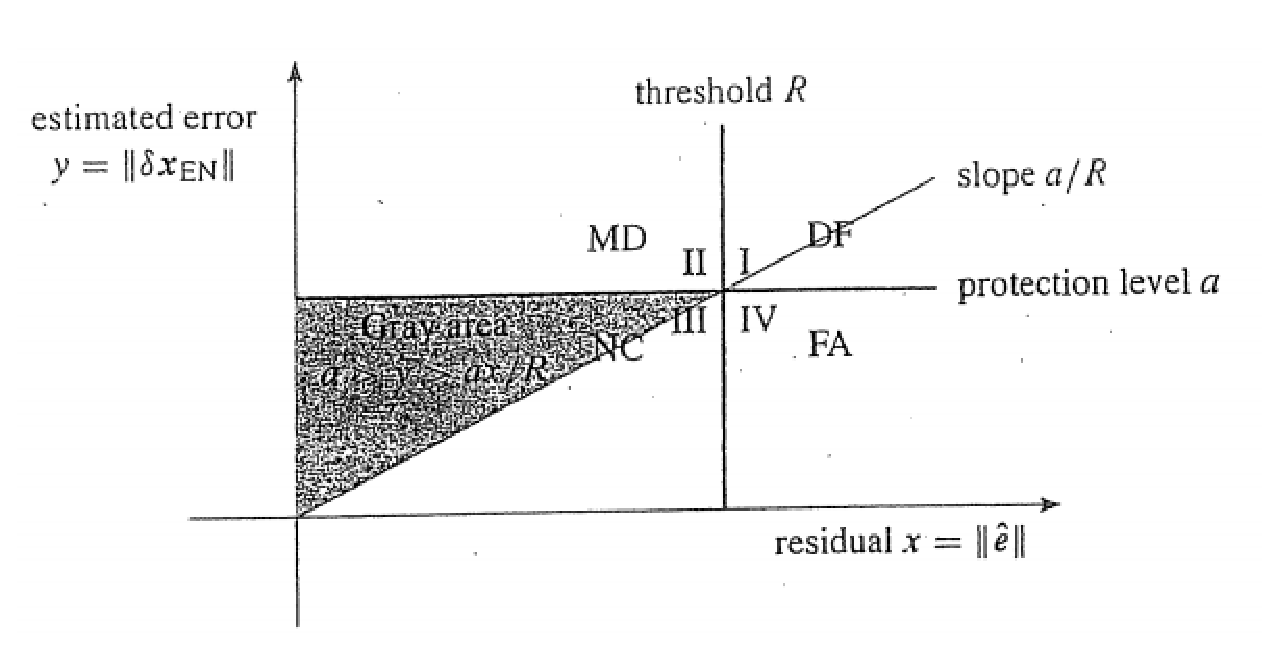
\includegraphics[width=0.7\linewidth]{TeX_files/Part03/chapter09/image/9-24}
			\caption{RAIM status, repeated. We aim for the gray area.}
			\label{fig:9-24}
		\end{figure}
		
		The failure mode axes in Figure \ref{fig:9-23} through the origin with slope $\alpha_i$are given exclusively from the geometry of the satellites and the receiver. The mode axis with largest $\aleph_i$is called $\alpha_max$ and the HPL is defined as
		\begin{equation}\label{eq:9.69}
			Horizontal\ Protection\ Level \quad HPL = \alpha_{max}\sigma_0
		\end{equation}
		
		where $\sigma_0$ is the a priori standard deviation of the pseudoranges \\$\sigma_0 = \sqrt{\hat{e}^T\sum^{-1}_b\hat{e}}/\sqrt{m-4}$.
		HPL is the radius of a circle in the horizontal plane,which is assured to contain the indicated horizontal position.
		
		The resulting RAIM fault detection algorithm is a simple one: Check the residual statistic to see if it is larger than the residual threshold R. If so, a system failure is declared.Given this simple algorithm, four outcomes are possible in Figures \ref{fig:9-21} and \ref{fig:9-24}.
		
		Under a normal condition (NC), the position error $\Arrowvert \delta x \Arrowvert $ does not exceed the protection level a and the residual is smaller than the threshold R, as in case III. If the position error does not exceed the protection level a, but the residual is larger than the threshold R,a false alarm (FA) has occurred, which is case IV. When both protection level and residual threshold have been breached, a detection failure (DF) has occurred— case I.Finally, a missed detection (MD) happens when the position error $\delta x$ is larger than the protection level a, but the residual is smaller than the residual threshold R; that is case II.
		
		When more than one failure mode exists, e in \ref{eq:9.66} has more than one non-zero component. We will not discuss that case. Brown $\&$ Hwang (1997) investigate RAIM in case of non-uniform weighted observations and multiple faults.
		
		Because the horizontal protection level depends on satellite geometry, it must be
		computed for each epoch and each position.
		
		Referring to Figure \ref{fig:9-24},we may introduce inequalities which characterize each region in the figure. For notational reasons in addition to the protection level a, we introduce the obvious new variables $x=\Arrowvert \hat{e} \Arrowvert$(norm of residual)and $y=\Arrowvert \delta x_{EN} \Arrowvert$(horizontal position error) such that $y=fx$ where $f= a/R$.
		
		A desired result will plot in the case III area, upper part, which is called normal operation. The inputs to RAIM are the variance $\sigma^2_b$ of a pseudorange observation, the coefficient matrix A of the linearized least-squares observation equations, and the maximum allowable probabilities for a false alarm P(FA) and a missed detection P(MD). The outputs are HPL and VPL.
		
		By the official definition at http://www.nstb.tc.faa.gov/Terms.html the Vertical Protection Level is half the length of a segment on the vertical axis, with its center at the true position, which is assured to contain the indicated vertical position.
		
		Further suggested reading is de Jong (1998), Kaplan $\&$ Hegarty (2006), and Nikiforov $\&$Roturier (2005).
	\subsection{easy14}\label{subsec:easy14}
		Some GPS applications generate long time series of position estimates. Most often, plotting the data produces a quick overview. However, it may be difficult from a plot to quantify statistical measures like mean value, standard deviation, and circular error probable.
		
		Our demonstrational sample is data collected on August 20, 2008 over a 4.2 hour period with a Thales DG16 static receiver at a site south of Aalborg. This commercial receiver can handle EGNOS data. However, there are dedicated EGNOS receivers that exploit the data in a more optimal manner. Plots from such receivers look more perfect than the ones produced by our DG16 receiver.
		
		The EGNOS corrected positions were computed by a MATLAB implementation at the Danish GPS Center (DGC). For a given alert limit a, EGNOS provides an integrity measure which advises whether or not to use the position in question.
		
		The EGNOS corrections can be obtained directly via the geostationary satellites listed in Table 9.8, or via a service called Signal in Space through the internet (SISNeT) or other services. In the present case we apply a postprocessing mode which relies on the EGNOS Message Server (EMS) at ftp://ems.estec.8sa.int/pub/
		
		In polar regions you may have difficulties in receiving signals from the geostationary satellites. Hence the internet version becomes useful. However, you may argue that the internet is not too often available near the poles!
		
		The complete EGNOS computation involves ionospheric and possibly tropospheric correction. The variance of the i th observation has four terms: a fast and long term contricorrection bution $\sigma^2_{flt}$ to range-rate correction (RRC), a tropospheric correction $\sigma^2_{tropo}$, an ionospheric correction $\sigma^2_{iono}$, and finally receiver noise and multipath $\sigma^2_{air}$:

		\begin{equation}\label{eq:9.70}
			\sigma^2_i = \sigma^2_{flt} + \sigma^2_{tropo} + \sigma^2_{iono} + \sigma^2_{air}.
		\end{equation}
		Typical values for a satellite with high elevation are $\sigma_{flt} = 0.26 m $, $\sigma_{tropo} = 0.01 m$, $\sigma_{iono} = 0.21 m$, and $\sigma_{air} = 3.26 m $. For a low elevation we might see $\sigma_{flt} = 0.55 m$ , $\sigma_{tropo} = 0.10 m$, $\sigma_{iono} = 0.91m$, and $\sigma_{air} = 3.28m$.

		Figure 9.25 shows the time series (deviations from mean values) for the three coordinates east, north, up at the location E. Positions computed from the raw pseudoranges (dark line) plot as noisy curves. Our MATLAB EGNOS correcting code (developed at DGC) was applied to the raw observations to produce less noisy curves (light). No smoothing is applied. A further quantification of the graphs in Figure 9.25 is added as Table 9.12. Figure 9.26 contains a plot of the corresponding horizontal positions.
	
		\begin{figure}
			\centering
			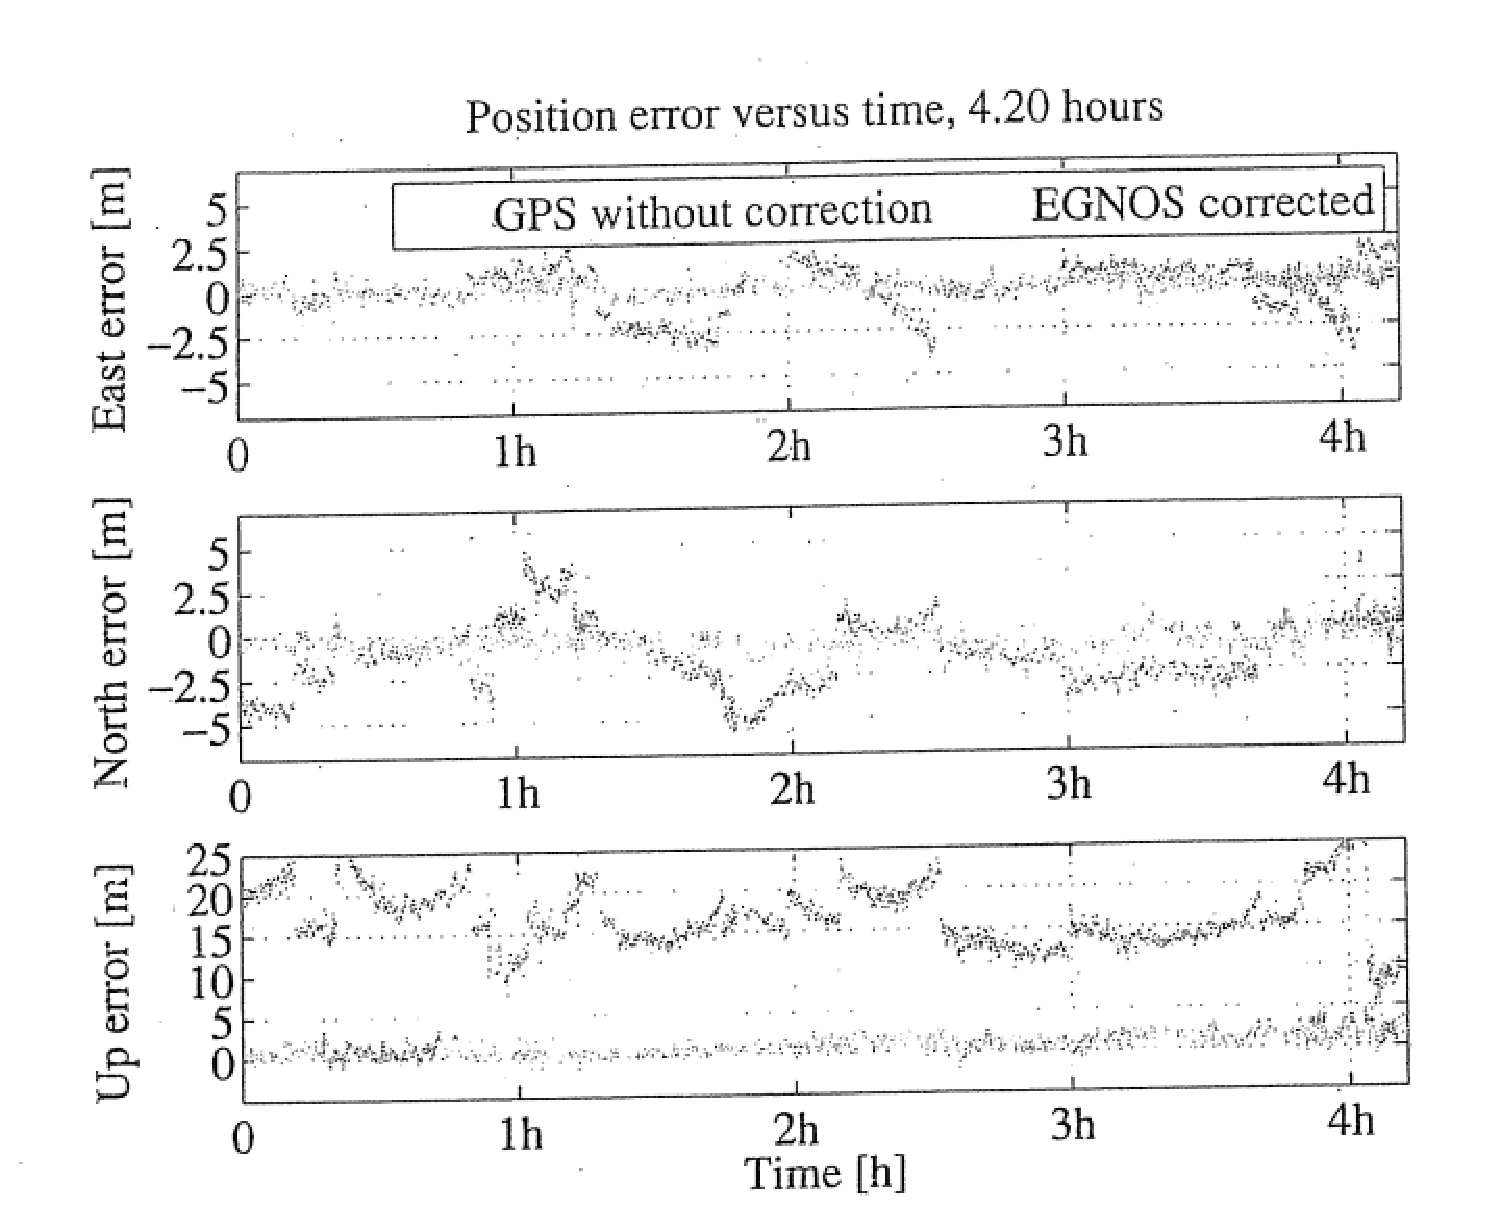
\includegraphics[width=0.7\linewidth]{TeX_files/Part03/chapter09/image/9-25}
			\caption{4.2 hours of data collected by a Thales DG16 receiver. The figure shows aast, north, up as computed from raw pseudoranges (dark) and from DGC EGNOS implemented correcting code (light).}
			\label{fig:9-25}
		\end{figure}
		
		Our script easy141 gives a recipe for computing Horizontal Protection Level (HPL) and Vertical Protection Level (VPL). We start from the coefficient matrix A for a single epoch
		
		\begin{equation}\label{eq:9.71}
			A = \begin{bmatrix}
				-\dfrac{X^1-X}{\rho^1} & -\dfrac{Y^1-Y}{\rho^1} & -\dfrac{Z^1-Z}{\rho^1} & 1 \\
				-\dfrac{X^2-X}{\rho^1} & -\dfrac{Y^2-Y}{\rho^1} & -\dfrac{Z^2-Z}{\rho^1} & 1 \\
				& \vdots & & \\
				-\dfrac{X^S-X}{\rho^S} & -\dfrac{Y^S-Y}{\rho^S} & -\dfrac{Z^S-Z}{\rho^S} & 1 \\
			\end{bmatrix}
		\end{equation}
		
		The larger script easy14 starts from a transformed version of A. The main change is to observe that $-\dfrac{X^i-X}{\rho^i} = \cos h^i \, \cos az^i$ where $h^i$ means the elevation angle and $az^i$ the azimuth of PRN i as seen from the receiver position.

		The first three columns of A contain the Euler angles between the line-of-sight and the (X , Y , Z) axes. However, we need those angles in the topocentric (E , N , U ) system.
		\begin{figure}[h]
			\centering
			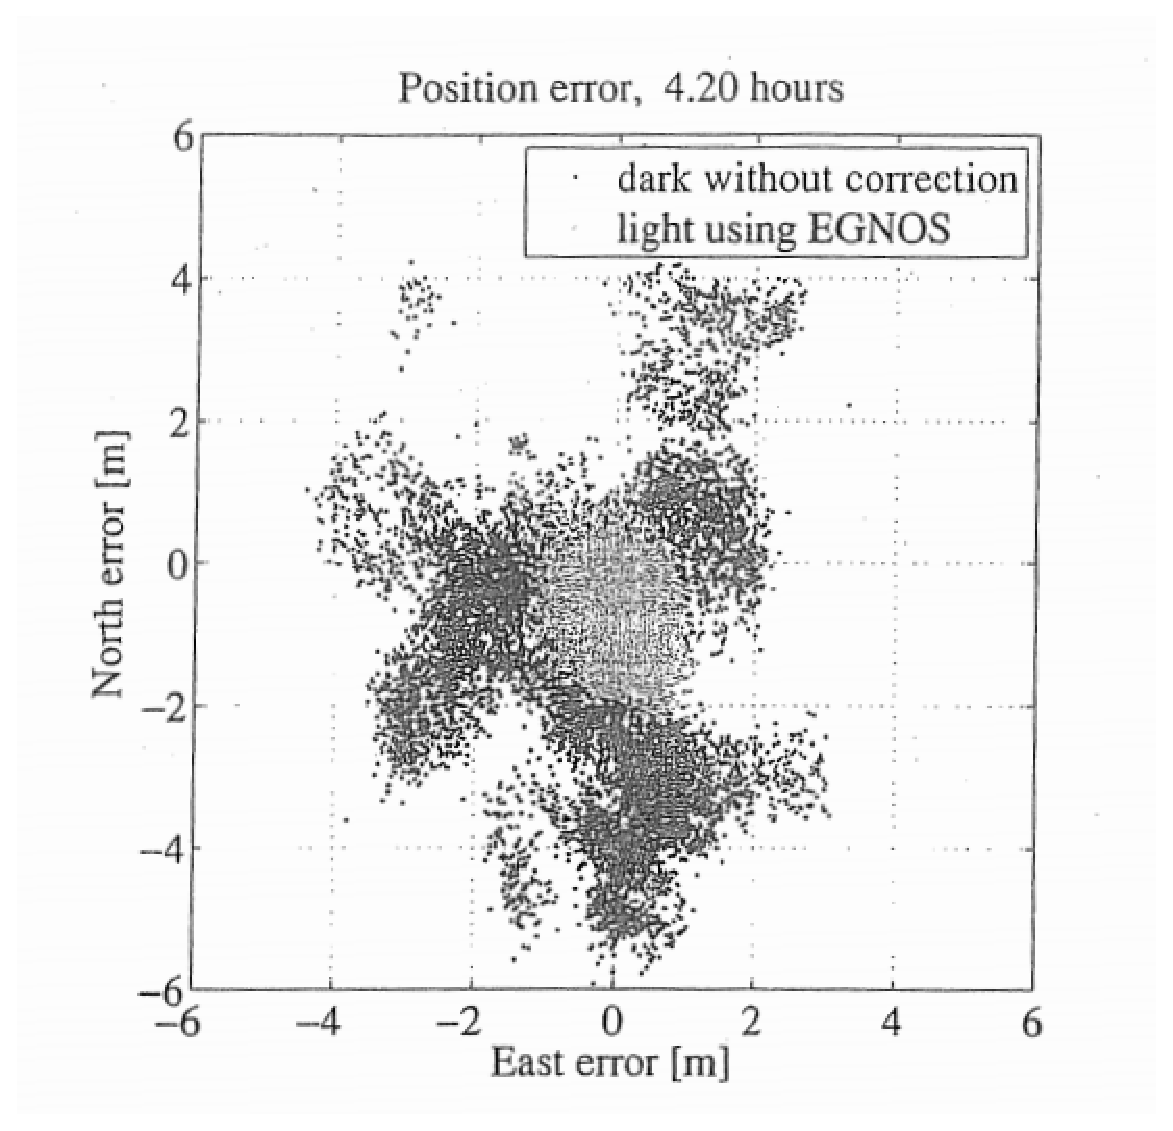
\includegraphics[width=0.7\linewidth]{TeX_files/Part03/chapter09/image/9-26}
			\caption{4.2 hours of data collected by a Thales DG16 receiver. The figure shows horizontal position errors in meters as computed from raw pseudoranges (dark) and much smoother result from DGC EGNOS implemented correcting code (light).}
			\label{fig:9-26}
		\end{figure}
		
		Denote row i of A by $-a_i$ for $i = 1,2\ldots,s.$ In equation(3.35) $-a_i$ was denoted by $\rho$.To transform from eocentric to topocentric coordinates, multiply columns 1 to 3 of A by $F = [ e\,n\,u ]$, see (9.64) and Figure 3.4:
		
		\begin{equation*}
			A(:,1:3)F = -
			\begin{bmatrix}
				a_1 \\ a_2 \\ \vdots
			\end{bmatrix}
			\begin{bmatrix}
				e & n & u
			\end{bmatrix} = -
			\begin{bmatrix}
				\cos h^1 \sin az^1 & \cos h^1 \cos az^1 & \sin h^1 \\
				\cos h^2 \sin az^2 & \cos h^2 \cos az^2 & \sin h^2 \\
                & \vdots & \\
				\cos h^s \sin az^s & \cos h^s \cos az^s & \sin h^s 
			\end{bmatrix}
		\end{equation*}
        This product, augmented with a column of ones, can also be computed directly as
		
		\begin{equation}\label{eq:9.72}
			B = \begin{bmatrix}
				\cos h^1 \sin az^1 & \cos h^1 \cos az^1 & \sin h^1 & 1 \\
				\cos h^2 \sin az^2 & \cos h^2 \cos az^2 & \sin h^2 & 1 \\
                & \vdots & & \\
				\cos h^s \sin az^s & \cos h^s \cos az^s & \sin h^s & 1 \\
			\end{bmatrix}
		\end{equation}
		The next steps involve simple expressions but heavy computational burdens. A weight matrix W for the observed pseudoranges is defined from the variances:
		
		\begin{equation}\label{eq:9.73}
			W = diag \begin{bmatrix}
			\sigma^{-2}_{1} & \sigma^{-2}_2 & \ldots & \sigma^{-2}_s
			\end{bmatrix}\: and \: \sum = (B^TWB)^{-1}
		\end{equation}
		\begin{tabular}{ccccccc}
			\hline 
			& CEP 50\% & CEP 95\% & $\rho_e$ & $\rho_n$ & $mean_e$ & $mean_n$ \\ 
			\hline 
			Raw pseudoranges & 1.8 & 3.8 & 1.3 & 1.8 & -0.2 & -1.4 \\ 
			DGC EGNOS corrected & 0.5 & 1.1 & 0.4 & 0.5 & 0.0 & -0.7 \\ 
			\hline 
		\end{tabular} 
		The entries $\sum_{11} = \sigma^2_1, \sum_{22} = \sigma^2_2,\: and \: \sum_{12} = \sum_{21} = \sigma_{12} $ of the covariancematrix $\sum$ constitute the coefficients in the equation for a confidence ellipse:
		
		\begin{equation*}
			\begin{bmatrix}
				x & y
			\end{bmatrix}\sum^{-1}
			\begin{bmatrix}
				x \\ y
			\end{bmatrix}
			= 1
		\end{equation*}
		The largest eigenvalue $\lambda$ of $\sum^{-1}$ is the semi-major axis of the confidence ellipse for the position solution
		\begin{equation*}
			\lambda_1 = \dfrac{1}{2}\left(\sigma^2_1 + \sigma^2_2 + \sqrt{(\sigma^2_1 + \sigma^2_2)^2 - 4(\sigma^2_1\sigma^2_2 - \sigma^2_{12})} \right)
		\end{equation*}
		compare equation(9.78) in Strang \& Borre(1997). The expression for $\lambda_1$ can be rewritten:
		\begin{equation}\label{9.74}
			\lambda_1 = \dfrac{\sigma^2_1 + \sigma^2_2}{2} + \sqrt{(\dfrac{\sigma^2_1 - \sigma^2_2}{2})^2 + \sigma^2_{12}}
		\end{equation}
		This version is found in RTCA/DO-229C (2001), page J.1.
		
		In a rotated coordinate system $(\xi,\eta)$, which diagonalizes $\sum$, we find
		\begin{equation}\label{9.75}
			\begin{bmatrix}
				\xi & \eta
			\end{bmatrix}
			\begin{bmatrix}
				\lambda_1 & 0 \\
				0 & \lambda_2
			\end{bmatrix}^{-1}
			\begin{bmatrix}
				\xi \\ \eta
			\end{bmatrix} = 1
		\end{equation}
		which is to be compared to (4.91).
		
		The EGNOS standard defines two magnification factors $K_H = norminv(1-1e-9,0,1)=6 $and$K_v = norminv(1-1e-7/2,0,1) = 5.33$. With $\sum_{33} = \sigma^2_{33}$ we finally obtain
		\begin{equation*}
			HPL = K_H\sqrt{\lambda_1}\: and \:VPL = K_V\sigma_{33}.
		\end{equation*}
		The EGNOS document also introduces its own non-precise HPL value which is 1.03 times larger than the HPL used here. Everything is implemented in easyl 41.
		
		We mention the general EGNOS objective in passing:
		\begin{itemize}
			\item the provision of integrity positioning with a safety-of-life quality,
			\item a better accuracy than GPS (down to about 1 to 2 m), and
			\item the possibility of establishing a geographical position with legal guarantees.
		\end{itemize}
		
		The safety-of-life service provides a horizontal accuracy of 4 m, a vertical accuracy of 8 m using the L1 and E5b frequencies, a timing accuracy of 30 ns in 95\% of the time, a time to alert of 6s, and a service availability of 99.5\%.
		\begin{figure}[h]
			\centering
			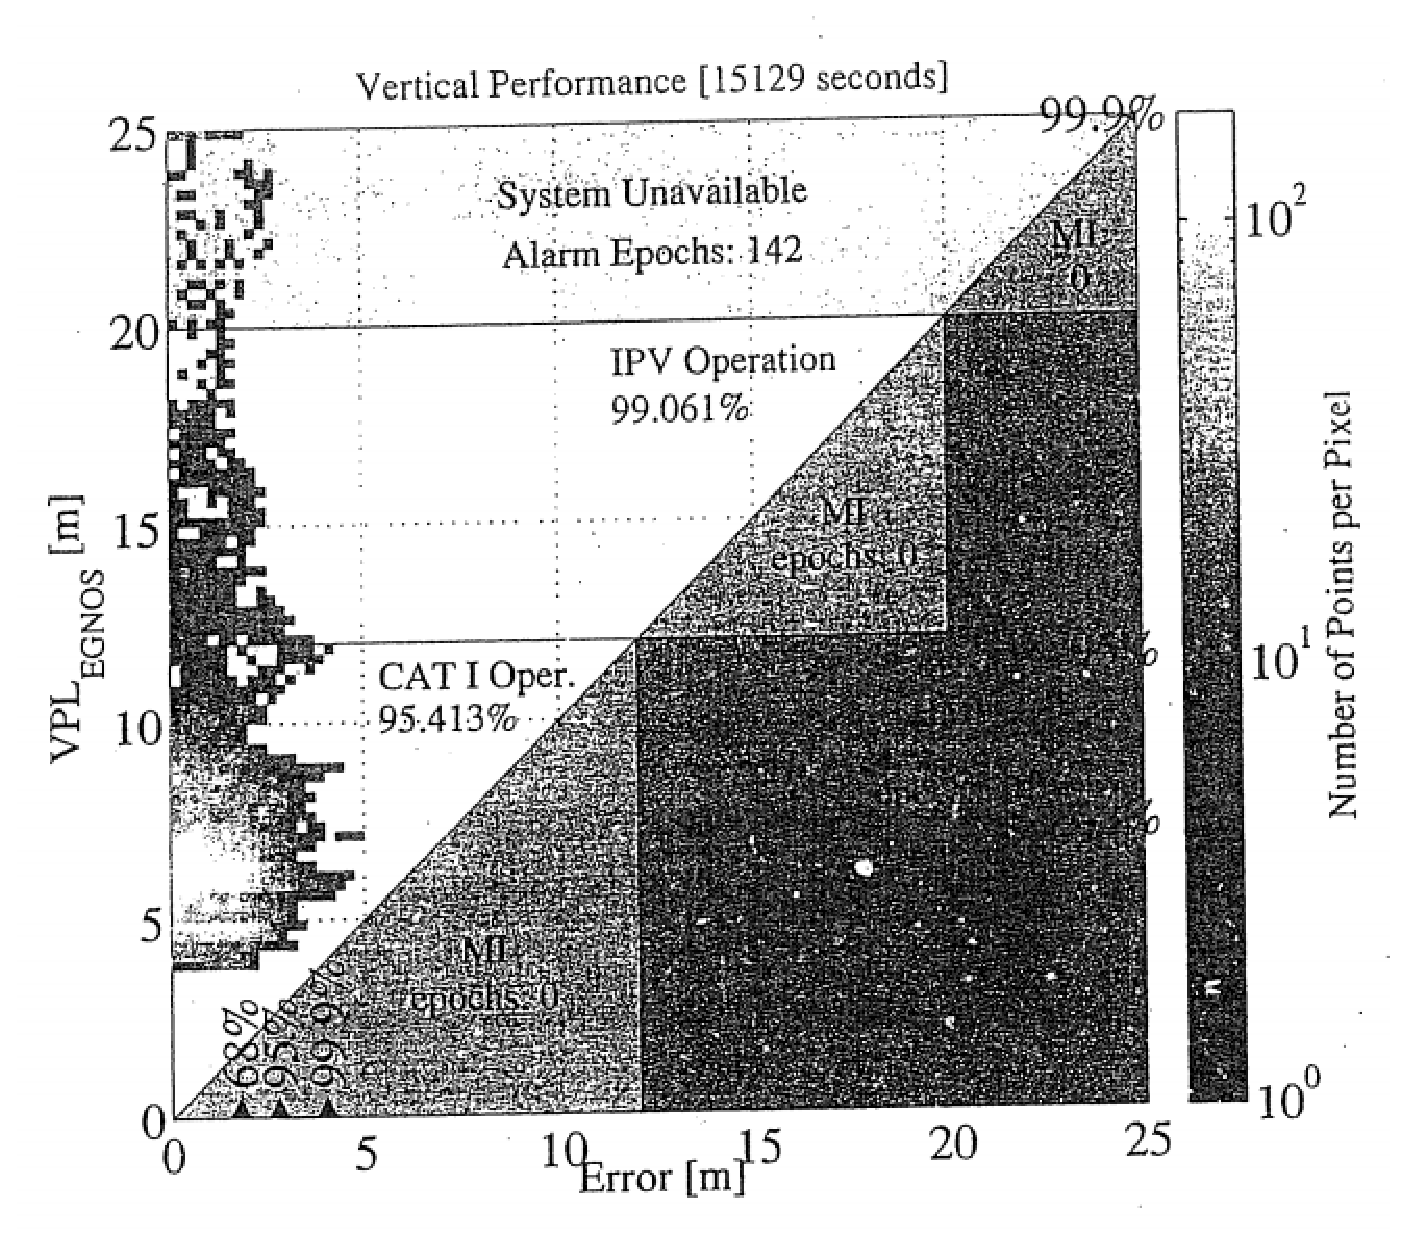
\includegraphics[width=0.7\linewidth]{TeX_files/Part03/chapter09/image/9-28}
			\caption{Positions depicted in Figure 9.25 are plotted versus vertical protection levels. Integrity failures happen in the areas marked HMI. The 20 m level corresponds to Instrument Precision with Vertical guidance (IPV). CAT I oper. corresponds to horizontal and vertical accuracies for precision landing for Category I (decision height 200feet). The lower and middle regions marked MI designate VPL failures. In the upper region marked MI, integrity and unavailability overlap.}
			\label{fig:9-28}
		\end{figure}
		Contemporary positioning theory uses the following four concepts which enter almost every specification: accuracy, integrity, continuity, and availability.
		
		Accuracy measures the difference between the (corrected) computed position and the true position. An SBAS implementation is obliged to quantify the accuracy of wide-area differentially corrected position. Accuracy may be estimated by the difference between computed and true position which, for CEP 95\%, is only exceeded 5\% of the time in the absence of system failures.
		
		Integrity risk is the probability that the SBAS exceeds either the instantaneous Horizontal or Vertical Alert Limit (HAL or VAL) and the system alert is silent beyond the time-toalarm. EGNOS has been designed for a 6-second time-to-alarm.
		
		Continuity and availability are expressed in global terms. If a blocked signal produces a system outage, this is not a global loss in continuity. It is a local phenomenon.
		
		\begin{figure}[h]
			\centering
			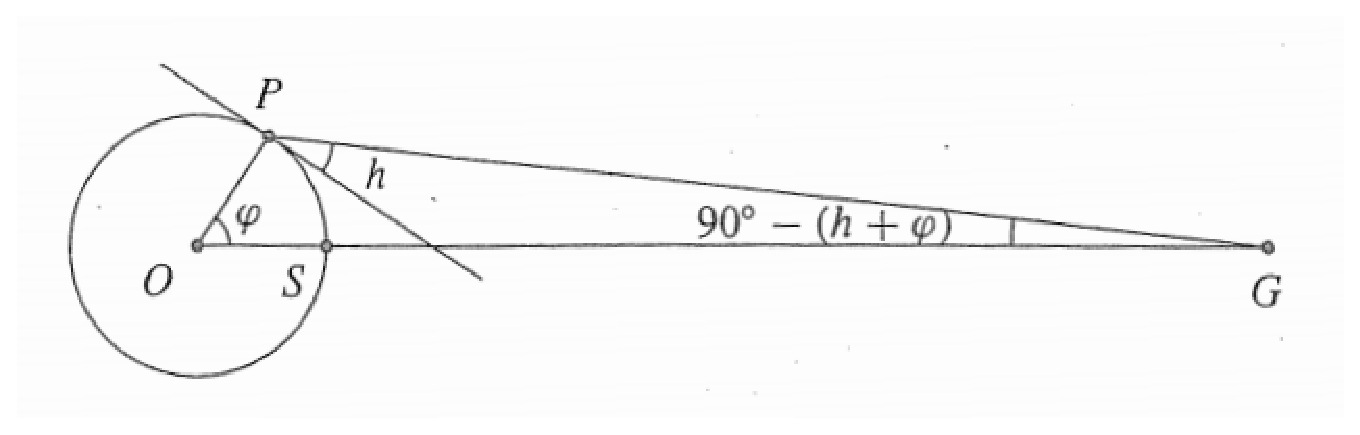
\includegraphics[width=0.7\linewidth]{TeX_files/Part03/chapter09/image/9-29}
			\caption{Elevation angle h to geostationary satellites as seen from the Earth’s surface as function of latitude $\varphi$ , spherical approximation.}
			\label{fig:9-29}
		\end{figure}
		
		A sophisticated plot was developed at Stanford University in 1998. The histogram of Figure 9.27 reports the horizontal system metrics provided by an EGNOS implementation done at DGC for a static user at Aalborg.
		
		The EGNOS concept only involves an alert limit a. The half line from (0, 0) through (a, a) partly limits the white area in which the attractive bins must lie!
		
		The horizontal axis indicates the error $\sqrt{e^2+n^2}$ in the SBAS navigation solution with respect to the surveyed antenna location. A more detailed discussion is presented in Tiberius \& Odijk (2008). The vertical axis indicates the protection level computed for every position solution. Each bin tabulates the occurrences of a specific pair(x, y)=(error,protection level). The color indicates the number of epochs in which that pair occurs. Note that the color scale is logarithmic and the bins are quantized into $0.25 \times 0.25m$squares.
		
		When HPL is larger than the alarm limit a , we experience a case of unavailability.The true error should always be less than the HPL. The long-term availability requirement of the SBAS is 99.9\% and hence at least 999 out of 1000 points should lie in the "Normal Operation" (USE) region. Here, the system maintained 99.7\% availability in horizontal positioning. It had 0.3\% unavailability (49 epochs out of 15 129).
		
		Availability can be associated with geostationary satellites only. In case you use the internet for obtaining the EGNOS information everything changes. In the present study we use EMS and not the real-time service SISNeT.
		
		
		Figure 9.28 shows the vertical system performance corresponding to the horizontal data presented above. The SBAS correction in the vertical dimension has poorer performance than the horizontal due to weaker geometry. The 12 m alert level corresponds to Category I landing and the 20 m level to Instrument Precision with Vertical guidance (IPV). The positioning system met all three safety metrics (accuracy, integrity, and continuity) with an
		availability of 99.061\%.
		\begin{figure}[h]
			\centering
			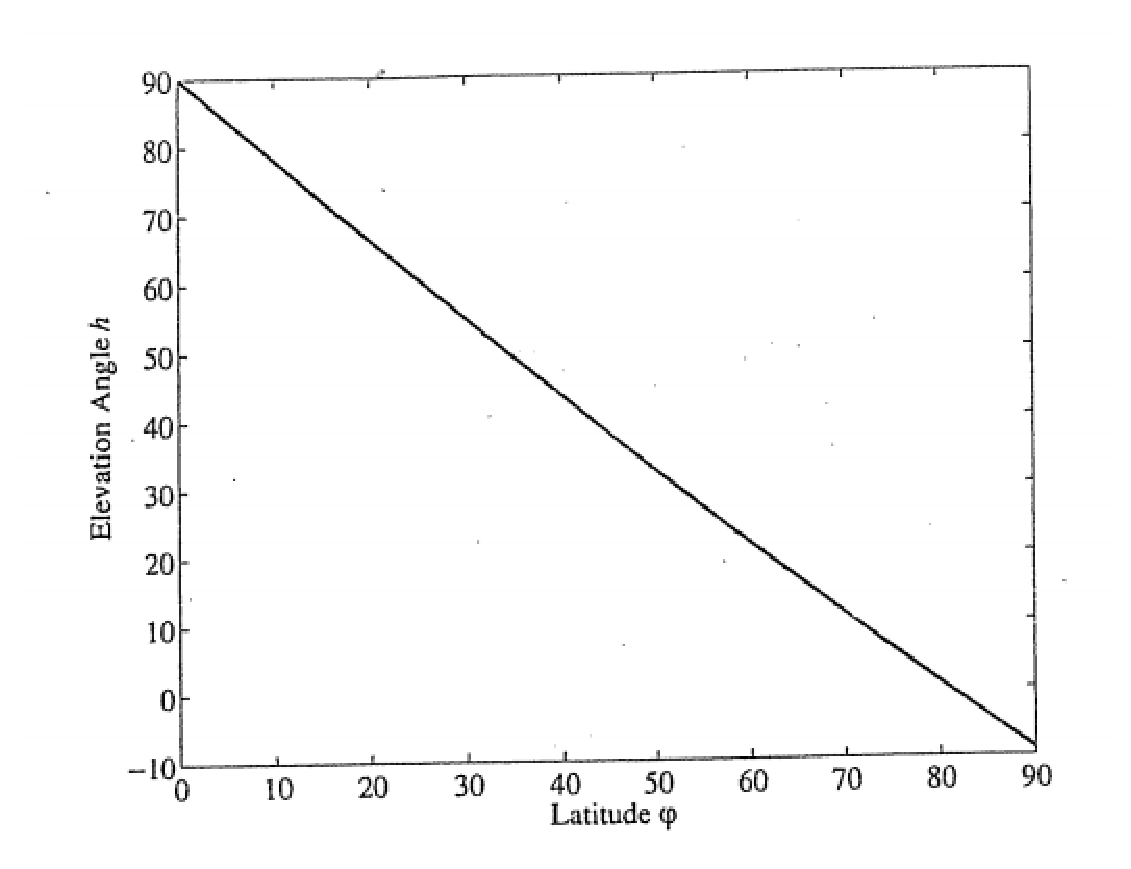
\includegraphics[width=0.7\linewidth]{TeX_files/Part03/chapter09/image/9-30}
			\caption{Elevation angle h to geostationary satellites as seen from the Earth’s surface}
			\label{fig:9-30}
		\end{figure}
		
		Kostas Dragunas added several changes to the original M-files vplstat and hplstat written by Todd Walter. The files are included with the permission of Stanford University.You also need the bound2 file in the download directory.
		
		We shall make a small digression to investigate the magnitude of the elevation angle h of a (geostationary) satellite as a function of the receiver site.
		
		Let a ground receiver have coordinates $(\varphi_E,\lambda_E)$ and let the sub-satellite coordinates be $(\varphi_S,\lambda_S)$. The geostationary satellite G, its sub-satellite point S , and the receiver site E define a plane. Let the Earth radius be $PO = a_E = 6371km$ and the distance between the geostationary satellite and the Earth center be $GO = a_G = 42486km$. With reference to Figure 9.29 we get, in a spherical approximation, for triangle OPG
		\begin{equation}\label{9.76}
			\dfrac{a_G}{\sin(\pi/2+h)} = \dfrac{a_E}{\sin(\pi/2-(h+\varphi))}.
		\end{equation}
		Some rewriting involving the addition formula for sines yields
		\begin{equation}\label{9.77}
			h = \arctan(\dfrac{\left| \cos \varphi - \dfrac{a_E}{a_G}\right| }{\sin \varphi})
		\end{equation}
		This angle is h = 0 for $\varphi$ = 80.9°; for $\varphi$ = 60.6° we get h — 20.9°, see Figure 9.30.
		
		
	\subsection{The Galileo Integrity Concept}
		GPS offers signals. Galileo offers services. This means that GPS signals are provided without any fee, while some Galileo services are commercial and supply encrypted navigation (data) messages containing additional integrity information.
		
		A network of forty Galileo Sensor Stations (GSS) shall permanently monitor signals from the Galileo satellites. GSS are similar to the tracking stations of GPS and to RIMS in EGNOS. 
		
		Observations taken at a GSS are transmitted in real time to the Galileo control center where the integrity data are created. Next these data are uploaded via nine uplink stations (ULS) to the satellites. Each Galileo satellite transmits a signal in space accuracy (SISA).SISA is the standard deviation of the difference between the true and the predicted values of position and clock. And SISA is based on prior values of SIS.
		
		A Galileo satellite is seen from s GSS $(s\leq8)$ with known coordinates. Let as usual A denote a matrix whose rows contain the components of a unit vector pointing from a GSS to satellite i, and let W be a diagonal matrix containing the weights of the observations;they may be elevation dependent. There are up to eight rows in A. A signal in space error(SISE) $\sigma_i$ for satellite i is computed as
		\begin{equation*}
			\sigma^2_i=(A^TWA)^{-1}
		\end{equation*}
		SISE is the important term in the integrity concept. It reflects the maximum error in SISA.In Galileo SISA has been designed to be less than 0.85 m.
		
		The signal in space monitoring accuracy (SISMA) is the standard deviation $\sigma_m$ of $\sigma_i$ :
		\begin{equation*}
			\sigma^2_m=max(a^T_i\sigma^2_ia_i)
		\end{equation*}
		where $a_i$ is a row vector containing the components of the unit vector pointing from the	receiver to satellite i. The threshold $T_i$ — which is to be compared to the alarm limit— is finally computed as
		\begin{equation}\label{eq:9.78}
			T_i=k_{fa}\sqrt{\sigma^2_i+\sigma^2_m}
		\end{equation}
		
		In case of no failure, a typical om is 0.7 m. For one failure to a GSS om = 1.3 m. For a maximum false alarm probability of $10^7$, $k_{fa}=norminv(1-1e-7,0)=5.2$and$T_i\approx6m$.
		
		Galileo is designed to deliver an alarm in case the error in the computed user position	exceeds an allowable level. This warning must be issued to the user within a given time (most often 6 s) with a given (high) probability. The integrity function provides a warning if the accuracy is not sufficient for the intended application. The update rate of the integrity information is 1 Hz. If the alarm limit is smaller than the threshold $T_i$, an alert is issued and the integrity flag is raised. If the alert limit is larger than $T_i$, no alert.
		
		There exist numerous papers on Galileo integrity. They illustrate various modifications of the above procedure. At the time of writing no final one is decided upon.
	
